\section{Single source}\label{ch:single_speaker_source}
To gain understanding about the interaction of several sources emitting sound simultaneously it is essential to first investigate the behaviour of a singular sound source. In the context of this project loudspeakers are investigated. The goal of this section is to find a way to represent the sound emission of loudspeakers within the frequencies boundaries of this project (\SIrange{60}{300}{\hertz}).
The representation must be suffiencently accurate yet relatively simple to calculate in order to be useful in the optimization process that is a later part of this project (see \autoref{ch:optimization}).

%This section aims to introduce and analyse the fundamental for a single source, by analyse the behaviour of a baffled circular plane piston source. The pressure around the piston source will be analysed analytically, to determine the radiation of a single speaker from \SI{60}{\hertz} and upwards and compare it with the measurement from \autoref{ch:polar_response}. The \SI{60}{\hertz} lower limit enable the simulation to be validated by measurement in the AAU anechoic chamber and is a used lower limit for the low/mid driver in some line source array \citep{V-DOSC}.  The analyse shall end out with a approximated simulation model of the \gls{dut}.
\subsection{Pressure emission from an omidirectional source}\label{ssec:omni}
As explained in \autoref{ch:polar_response} loudspeakers are commonly treated as omnidirectional sources at low frequencies. Taking advantage of this approximation, the sound pressure emission in free field conditions can be described conveniently. \citep[p. 171]{Kinsler2000} state the following equation \autoref{eq:omni_source} for a pulsating sphere. It has to be noted, that the position of the sphere in the given case is the acoustic center of the loudspeaker (see \autoref{sec:ac_center}).
\begin{equation}\label{eq:omni_source}
p(r,t)\,=\,\rho_0 c V_0 \left(\frac{a}{r}\right)\cos \theta_a \textbf{\textit{e}}^{j\left(\omega t - k(r-a)+\theta_a\right)}
\end{equation}
\startexplain
\explain{$p$ is the sound pressure.}{\si{\pascal}}
\explain{$r$ is the distance, for which the pressure is being calculated, \(r>a\).}{\si{\meter}}
\explain{$t$ is the time, for which the pressure is being calculated.}{\si{\meter}}
\explain{$\rho_0$ is the specific density of air.}{\si{\kilo\gram\per\cubic\meter}}
\explain{$c$ is the speed of sound.}{\si{\meter\per\second}}
\explain{$V_0$ ist the peak velocity at the surface of the spherical source.}{\si{\meter\per\second}}
\explain{$a$ is the radius of the spherical source.}{\si{\meter}}
\explain{$\theta_a$ is equal to $\tan(ka)$.}{\si{1}}
\explain{$\omega$ is the angular frequency.}{\si{\second^{-1}}}
\explain{$k$ is the wavenumber.}{\si{\meter^{-1}}}
\stopexplain

\subsection{Pressure emission from a baffled piston}\label{ssec:piston}
Another  approach to analytically approximate the behaviour of a cone loudspeaker is given by \citep[p. 179 ff.]{Kinsler2000}, where the behaviour of the sound radiated from a plane circular piston surrounded by an infinte rigid baffle is described. The piston model is derived from the model of a continous line source as described in \citep[p. 176 f.]{Kinsler2000}.


%To characterize the directional properties of an analytical model of the \gls{dut}, the source will be modulated in two dimension as one baffled circular plane piston source. The analysis of a piston source in two dimension built on a thin piston source in three dimension where the x axis is fixed in the plot. This is possible because of vertical beam patten symmetry of \autoref{fig:continues_line_source} \citep{Kinsler2000}. The piston lays flat down so i look like a line source and have radius $a$. The baffled circular plane piston source can be considered as many continuous line sources, which detonate dx and is pointing towards the reader on \autoref{fig:continues_line_source}. The calculated pressure point will be in far field where $r>>a$ holds and the surface integral can be rewritten to a Bessel function \citep{Kinsler2000}. The pressure formula is therefore:

\begin{equation}\label{eq:piston_source}
p(r,\theta ,t)=\frac{j}{2} \rho_{0}c  V_{0}\frac{a}{r}ka \left ( \frac{2J_1(ka\, sin(\theta ))}{ka\, sin(\theta )} \right )e^{j(\omega t-kr)}
\end{equation}
\startexplain
	\explain{$r$ is the distance, for which the pressure is being calculated, \(r>a\).}{\si{\meter}}
	\explain{$\theta$ is the angle at which the pressure is calculated, relative to the direction, in which the piston is moving.}{\si{1}}
	\explain{$t$ is the time, for which the pressure is being calculated.}{\si{\meter}}
	\explain{$j$ is the imaginary unit}{\si{1}}
	\explain{$\rho_0$ is the specific density of air.}{\si{\kilo\gram\per\cubic\meter}}
	\explain{$c$ is the speed of sound.}{\si{\meter\per\second}}
	\explain{$V_0$ ist the peak velocity of the piston.}{\si{\meter\per\second}}
	\explain{$a$ is the radius of the piston.}{\si{\meter}}
	\explain{$k$ is the wavenumber.}{\si{\meter^{-1}}}
	\explain{$J_1$ is the Bessel function of the first kind of order 1.}{\si{1}}
	\explain{$\omega$ is the angular frequency.}{\si{\second^{-1}}}
\stopexplain

A major disadvantage to utlizing the piston model in the context of the project is, that no information about the cabinet of the \gls{dut} is incorporated. The concept of an infinite rigid baffle leads to results that are axis symmetric along the \SIrange{-90}{90}{\degree}-line in a polar plot. This is illustrated in \autoref{fig:piston_analytical}.
\begin{figure}[H]
	\centering
	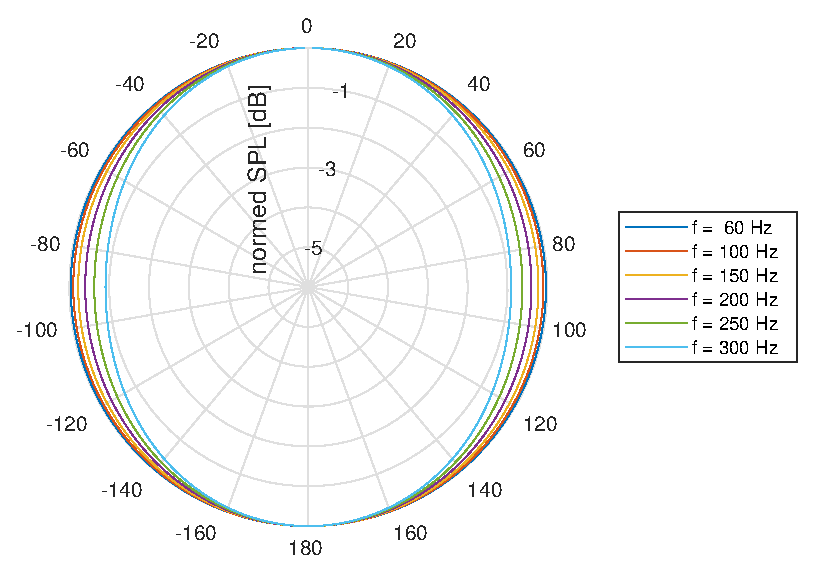
\includegraphics[width=0.7\textwidth]{piston.eps}
	\caption{normed SPL according to \autoref{eq:piston_source}, $a=165.3$\si{\milli\meter}$\,\approx 13$'', corresponding to the size of \citep{seas33}.}
		\label{fig:piston_analytical}
\end{figure}
\autoref{fig:piston_analytical} displays almost perfect omnidirectional behaviour for lower frequencies and lowering pressure towards $\pm$\SI{90}{\degree} for higher frequencies. The deviation from omnidirectionality has the same qualitative appearance as the measured pressure curves in \autoref{fig:03_02_pressure_main}, however they significantly differ in numbers.
\begin{figure}[htbp]
	\centering
	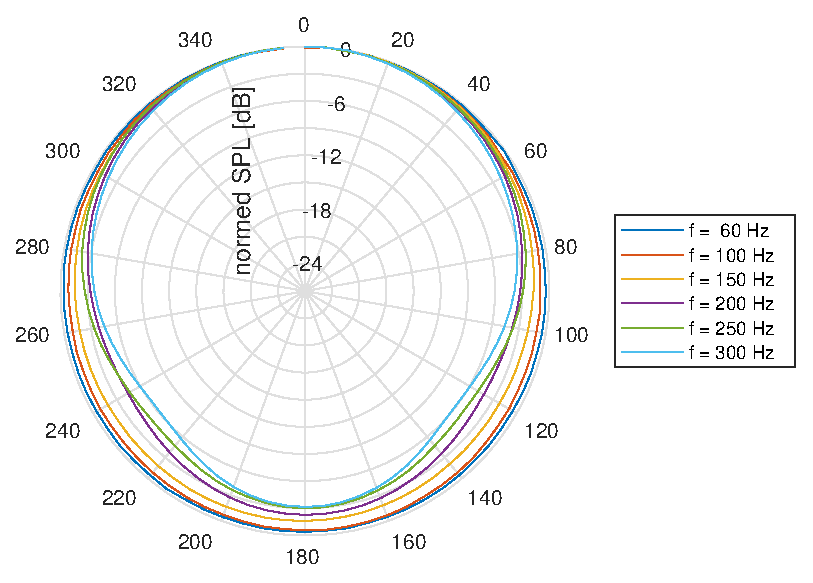
\includegraphics[width=0.7\textwidth]{03_02_meas1_pressure.eps}
	\caption{Normed \gls{spl}, measured at a distance \(d=\)\SI{2.74}{\meter}, see Appendix \ref{ax:directional_2}}
		\label{fig:03_02_pressure_main}
\end{figure}
\autoref{fig:03_02_pressure_main} also illustrates, that the solutions obtained with \autoref{eq:piston_source} do not realistically represent how the pressure is emitted on the back side of the speaker. Specifically, the indents in the in the curves for frequencies $\ge$\SI{200}{\hertz} at approx. $\pm$\SI{125}{\hertz} in \autoref{fig:03_02_pressure_main} deviate from the shape that is drawn by the piston model.
%The movement of the surface is described with

%\begin{equation}
%v = V_{0} \cdot exp(j \omega t)
%\end{equation}

%\startexplain
%    	\explain{$v$ is the complex speed of the line source }{\si{1}}
%        \explain{$V_{0}$ is the Amplitude}{\si{1}}
%        \explain{$j$ is the imaginary unit }{\si{1}}
%        \explain{$\omega$ is the angular velocity }{\si{1}}
%        \explain{$t$ is the time }{\si{1}}
%\stopexplain
    
%Each small sources is treated as an baffled simple source with a width of $dx$ and the source strange can be modulated as following      
%
%\begin{equation}
%dQ = V_{0} 2 a\, sin(\phi) \, dx
%\end{equation}
%
%    \startexplain
%    		\explain{$dQ$ is the simple source strange }{\si{1}}
%        \explain{$V_{0}$ is the Amplitude}{\si{1}}
%        \explain{$a$ is the radius for cylinder }{\si{1}}
%        \explain{$\phi$ is the angle between the radius $a$ and the x axis}{\si{1}}
%        \explain{$dx$ is the length for the simple source }{\si{1}}
%    \stopexplain    
% 
%The following \autoref{fig:continues_line_source} shows an example of the continues line source where one of the small source is showed with width $dx$ and length $2a \, sin(\phi)$. 
%
%\begin{figure}[H]
%	\centering
%\begin{picture}(0,0)%
%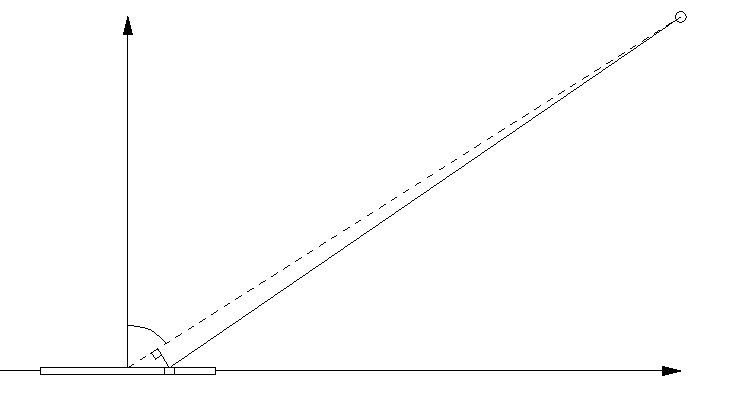
\includegraphics{line_source.pdf}%
%\end{picture}%
%\setlength{\unitlength}{746sp}%
%%
%\begingroup\makeatletter\ifx\SetFigFont\undefined%
%\gdef\SetFigFont#1#2#3#4#5{%
%  \reset@font\fontsize{#1}{#2pt}%
%  \fontfamily{#3}\fontseries{#4}\fontshape{#5}%
%  \selectfont}%
%\fi\endgroup%
%\begin{picture}(31223,16833)(-5411,-436)
%\put(12106,7139){r'}%
%\put(24121,15599){P(r,$\theta$,t)}%
%\put(946,2684){$\theta$}%
%\put(23851,659){x}%
%\put(-89,16094){z}%
%\put(11341,8354){r}%
%\put(3466,-571){$a$}%
%\put(1441,-376){$dx$}%
%\put(-134,-421){0}%
%\put(-4049,-571){$-a$}%
%\put(226,1649){$\Delta$r}%
%\end{picture}%
%	\caption{The model of a continues line source where y axis is pointing towards the reader. (ref the book)}
%		\label{fig:continues_line_source}
%\end{figure}




%\subsection{Comparison: calculations based on the baffled piston and measured polar respone}
%In this section, the \gls{dut} will be simulated as a baffled circular plane piston source as described in \autoref{ch:single_speaker_source} and compared to the actually measurement of the \gls{dut} \autoref{ax:directional_2}. An piston simulated model of \citep{seas33} in MATLAB shows in \autoref{fig:piston_model_of_seas33}
%
%\begin{figure}[H]
%	\centering
%	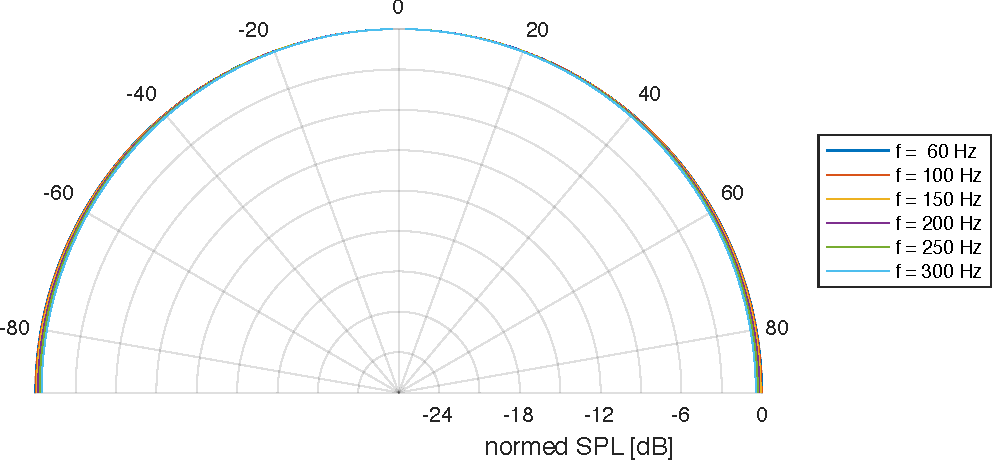
\includegraphics[width=0.8\textwidth]{piston_model.pdf}
%	\caption{The figure shows  The \gls{dut} which correspond to this figure is a \citep{seas33}}
%		\label{fig:piston_model_of_seas33}
%\end{figure}
%
%The actually measurement of the \citep{seas33}  \autoref{ax:directional_2}.
%
%\begin{figure}[H]
%	\centering
%	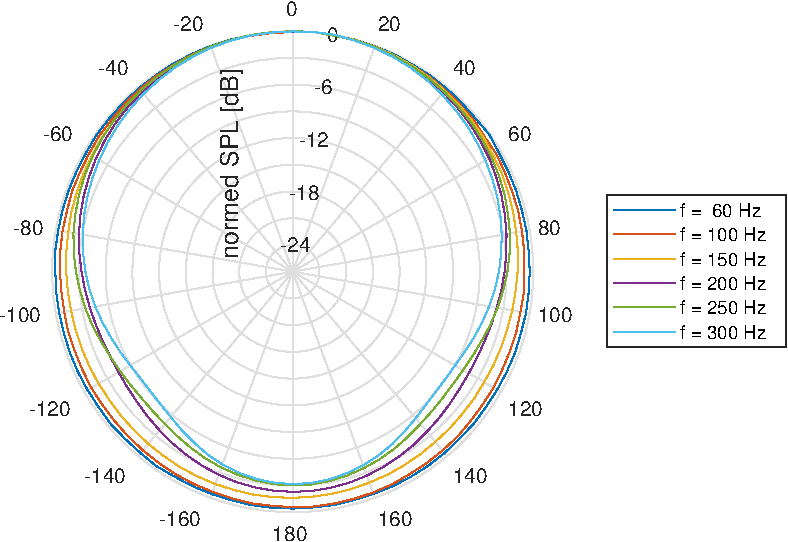
\includegraphics[width=0.8\textwidth]{meas1_seas.pdf}
%	\caption{The figure shows  The \gls{dut} which correspond to this figure is a \citep{seas33}}
%		\label{fig:speaker_model}
%\end{figure}

\subsection{Fitting the omnidirectional source model to the \gls{dut}}\label{sec:correction}
The analytical descriptions of both the pulsating sphere (see \autoref{ssec:omni}) and the piston (see \autoref{ssec:piston}) do not describe the measured behaviour of the \gls{dut} in an adequate manner. In order to be able to perfom an optimization of the signal processing parameters for the speaker array (see \autoref{ch:optimization}), a sufficient model has to be obtained. For the sake of this project, it has been chosen to rely on measured data.
As the pressure and phase characteristic of the \gls{dut} have been ascertained in measurements (see Appendices \ref{ax:directional_1},\ref{ax:directional_2}), the measurements results can be processed to obtain a correction table relating to the model of the omnidirectional source. This is achieved by calculating a difference of the measured data from the ideal values, that would suggest omnidirectionality at any given frequency. The resolution of the correction grid is determined by angular resolution and the frequency resolution of the polar response measurement, that it is based on.  \autoref{fig:correction_3d} shows a pressure correction grid, based on the polar response from Appendix \ref{ax:directional_2}.
\begin{figure}[H]
	\centering
	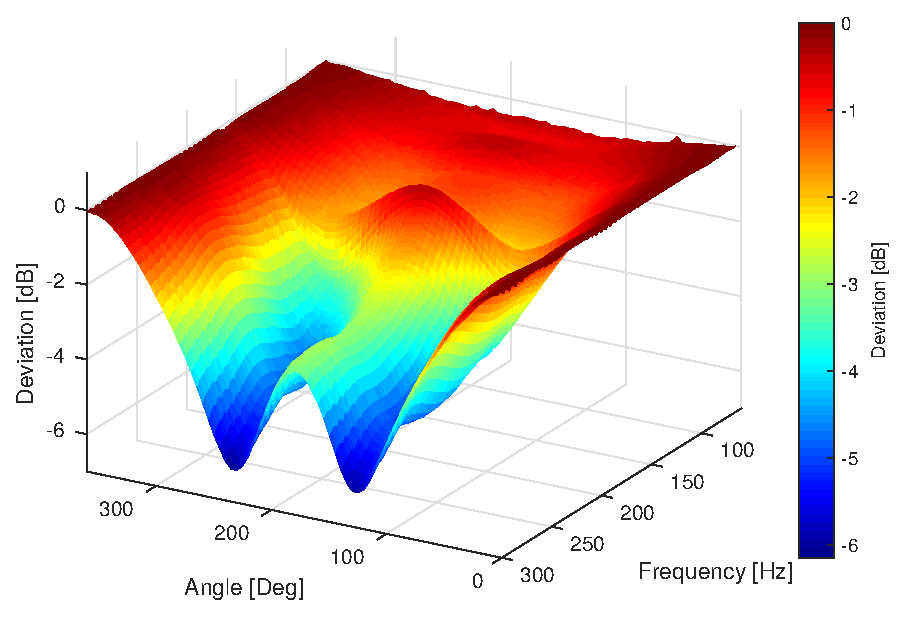
\includegraphics[width=0.7\textwidth]{correction_3d.eps}
	\caption{Pressure correction data, based on measurement data from Appendix \ref{ax:directional_2}}
		\label{fig:correction_3d}
\end{figure}
With the correction values applied, an augmented form of \autoref{eq:omni_source} can be established. Note, that while the deviation from omnidirectionality is visualized in \autoref{fig:correction_3d} in a \si{\decibel}-scale, for the usage in the \textsf{Dev}-function in \autoref{eq:aug_omni}, data has to be presented linearly.
\begin{equation}\label{eq:aug_omni}
p(r,t)\,=\,\rho_0 c V_0 \left(\frac{a}{r}\right)\cos \theta_a \textbf{\textit{e}}^{j\left(\omega t - k(r-a)+\theta_a\right)}\cdot\textsf{Dev}(f,\phi)
\end{equation}
\startexplain
\explain{$p$ is the sound pressure.}{\si{\pascal}}
\explain{$r$ is the distance, for which the pressure is being calculated, \(r>a\).}{\si{\meter}}
\explain{$t$ is the time, for which the pressure is being calculated.}{\si{\meter}}
\explain{$\rho_0$ is the specific density of air.}{\si{\kilo\gram\per\cubic\meter}}
\explain{$c$ is the speed of sound.}{\si{\meter\per\second}}
\explain{$V_0$ ist the peak velocity at the surface of the spherical source.}{\si{\meter\per\second}}
\explain{$a$ is the radius of the spherical source.}{\si{\meter}}
\explain{$\theta_a$ is equal to $\tan(ka)$.}{\si{1}}
\explain{$\omega$ is the angular frequency.}{\si{\second^{-1}}}
\explain{$k$ is the wavenumber.}{\si{\meter^{-1}}}
\explain{$\textsf{Dev}$ is the pressure deviation from the correction table.}{\si{1}}
\explain{$f$ is the frequency.}{\si{\hertz}}
\explain{$\phi$ is the angle, for which the pressure is being calculated relative to the main axis of the speaker.}{\si{1}}
\stopexplain
\subsection{Conclusion}
Investigating analytical ways to express the behaviour of a speaker by incorporation no other information then its size leads to results that are not particulary accurate and are therefore of limited use. While it appears to be possible to get better estimates by incorporating more information into a numerical model (e.g. \citep{vanderkooy10}). The given objective of using the model for an optimization makes this approach unfeasible. Because measurements have been conducte investigating the directional characteristics of the loudspeaker that will later be used, a more empirical approach has been found. Exploiting information from the measurements, the relatively simple model of a pulsating sphere can be augmented, so that it fits the behaviour of the \gls{dut}.